% Options for packages loaded elsewhere
\PassOptionsToPackage{unicode}{hyperref}
\PassOptionsToPackage{hyphens}{url}
\PassOptionsToPackage{dvipsnames,svgnames*,x11names*}{xcolor}
%
\documentclass[
  a4paper,
  10pt]{article}
\usepackage{amsmath,amssymb}
\usepackage{lmodern}
\usepackage{iftex}
\ifPDFTeX
  \usepackage[T1]{fontenc}
  \usepackage[utf8]{inputenc}
  \usepackage{textcomp} % provide euro and other symbols
\else % if luatex or xetex
  \usepackage{unicode-math}
  \defaultfontfeatures{Scale=MatchLowercase}
  \defaultfontfeatures[\rmfamily]{Ligatures=TeX,Scale=1}
\fi
% Use upquote if available, for straight quotes in verbatim environments
\IfFileExists{upquote.sty}{\usepackage{upquote}}{}
\IfFileExists{microtype.sty}{% use microtype if available
  \usepackage[]{microtype}
  \UseMicrotypeSet[protrusion]{basicmath} % disable protrusion for tt fonts
}{}
\makeatletter
\@ifundefined{KOMAClassName}{% if non-KOMA class
  \IfFileExists{parskip.sty}{%
    \usepackage{parskip}
  }{% else
    \setlength{\parindent}{0pt}
    \setlength{\parskip}{6pt plus 2pt minus 1pt}}
}{% if KOMA class
  \KOMAoptions{parskip=half}}
\makeatother
\usepackage{xcolor}
\IfFileExists{xurl.sty}{\usepackage{xurl}}{} % add URL line breaks if available
\IfFileExists{bookmark.sty}{\usepackage{bookmark}}{\usepackage{hyperref}}
\hypersetup{
  pdftitle={Spectral element method and discrete operators},
  pdfauthor={A. Perez; A. V. Mohanan; M. Moniri; Z. Yuan},
  pdfkeywords={Templates, Talk},
  colorlinks=true,
  linkcolor={blue},
  filecolor={Maroon},
  citecolor={blue},
  urlcolor={blue},
  pdfcreator={LaTeX via pandoc}}
\urlstyle{same} % disable monospaced font for URLs
\usepackage{listings}
\newcommand{\passthrough}[1]{#1}
\lstset{defaultdialect=[5.3]Lua}
\lstset{defaultdialect=[x86masm]Assembler}
\usepackage{graphicx}
\makeatletter
\def\maxwidth{\ifdim\Gin@nat@width>\linewidth\linewidth\else\Gin@nat@width\fi}
\def\maxheight{\ifdim\Gin@nat@height>\textheight\textheight\else\Gin@nat@height\fi}
\makeatother
% Scale images if necessary, so that they will not overflow the page
% margins by default, and it is still possible to overwrite the defaults
% using explicit options in \includegraphics[width, height, ...]{}
\setkeys{Gin}{width=\maxwidth,height=\maxheight,keepaspectratio}
% Set default figure placement to htbp
\makeatletter
\def\fps@figure{htbp}
\makeatother
\setlength{\emergencystretch}{3em} % prevent overfull lines
\providecommand{\tightlist}{%
  \setlength{\itemsep}{0pt}\setlength{\parskip}{0pt}}
\setcounter{secnumdepth}{-\maxdimen} % remove section numbering
\usepackage[utf8]{inputenc}
\usepackage{amsmath}
\usepackage{amsfonts}
\usepackage{amssymb}
\usepackage{listings}
\usepackage{tikz}
% \usepackage{pgfplots}
\usepackage{lipsum}
\usepackage{algorithm,algpseudocode}

\lstset{ %%%%%%
  language=Fortran,
  belowskip=-0.9 \baselineskip,
  keywordstyle=\bfseries,
  basicstyle=\footnotesize,        % the size of the fonts that are used for the code
  breakatwhitespace=false,         % sets if automatic breaks should only happen at whitespace
  breaklines=true,                 % sets automatic line breaking
  captionpos=b,                    % sets the caption-position to bottom
  deletekeywords={...},            % if you want to delete keywords from the given language
  extendedchars=true,              % lets you use non-ASCII characters; for 8-bits encodings only, does not work with UTF-8
  frame=lines,	                   % adds a frame around the code
  keepspaces=true,                 % keeps spaces in text, useful for keeping indentation of code (possibly needs columns=flexible)
  showspaces=false,                % show spaces everywhere adding particular underscores; it overrides 'showstringspaces'
  showstringspaces=false,          % underline spaces within strings only
  showtabs=false,                  % show tabs within strings adding particular underscores
  stepnumber=2,                    % the step between two line-numbers. If it's 1, each line will be numbered
  tabsize=2,	                    % sets default tabsize to 2 spaces
  title=\lstname,                   % show the filename of files included with \lstinputlisting; also try caption instead of title
  }

\ifLuaTeX
  \usepackage{selnolig}  % disable illegal ligatures
\fi
\usepackage[]{natbib}
\bibliographystyle{plainnat}

\title{Spectral element method and discrete operators}
\author{A. Perez \and A. V. Mohanan \and M. Moniri \and Z. Yuan}
\date{April 13, 2021}

\begin{document}
\maketitle
\begin{abstract}
Report of the topics covered by groups G01 and G02. The report was made
collaboratively by the authors in an
\href{https://hackmd.io/@jmtW1K-nT5O31NGGrCd6Pg/ByZNQkZH_}{online HackMD
document} with accompanying
\href{https://hackmd.io/@ashwinvis/B1PY2JorO}{presentation}
\end{abstract}

\hypertarget{continuous-galerkin-formulation}{%
\section{Continuous Galerkin
formulation}\label{continuous-galerkin-formulation}}

Based on posing problems in their variational (weak) form which is an
equivalent integral form to that of their classical representation. Take
advection-diffusion equation as an example: expressed in strong form as
\begin{equation}
\frac{\partial{u}}{\partial{t}} + c \frac{\partial{u}}{\partial{x}} =  \nu \frac{\partial^{2}u}{\partial{x}^{2}}.
\end{equation}

A \textbf{residual} can be defined as: \begin{equation}
L=\frac{\partial{u}}{\partial{t}} + c \frac{\partial{u}}{\partial{x}} -  \nu \frac{\partial^{2}u}{\partial{x}^{2}}.
\end{equation}

The weak form is
obtained by multiplying the residual by a \textbf{test function}
\(v(x)\) and integrating over the domain: \begin{equation}
(v,L)=\int_{\Omega} v(\frac{\partial{u}}{\partial{t}} + c \frac{\partial{u}}{\partial{x}} -  \nu \frac{\partial^{2}u}{\partial{x}^{2}})dx=0.
\end{equation}

The order of the second derivative in the diffusion term can be reduced
by integrating by parts:

\begin{align}
\int_{\Omega} (v\frac{\partial u}{\partial t} + cv\frac{\partial u}{\partial x} + \nu\frac{\partial v}{\partial x}\frac{\partial u}{\partial x})dx + [v\frac{\partial u}{\partial x}]_{\partial\Omega}) = 0,
\end{align}

by choosing a basis \(v(x)\) that vanishes at the boundaries of the
domain \(\partial\Omega\). The Galerkin formulation is then the
following.

Find \(u\) such that: \begin{align}
\int_{\Omega} (v\frac{\partial u}{\partial t} + cv\frac{\partial u}{\partial x} + \nu\frac{\partial v}{\partial x}\frac{\partial u}{\partial x})dx = 0.
\end{align}

A potential candidate for \(u(x,t)\) can be represented by a combination
of \textbf{trial functions} \(\psi\) such that: \begin{equation}
    u_N(x,t) = \sum_{n=0}^N u_n(t) \psi_n(x) = \underline{\psi}(x)^T \cdot \underline{u}(t),
\end{equation}

where \(\underline{\psi}(x)\) and \(\underline{u}\) are the column vectors for the basis functions and the coefficients. In the Galerkin method, the test function \(v(x)\) can also be
represented by the same set of trial functions.

\begin{equation}
    v(x) = \sum_{n=0}^N v_n \psi_n(x) = \underline{\psi}(x)^T \cdot \underline{v}.
\end{equation}

Applying this to the weak formulation of the Advection/Diffusion
equation and considering \(c=\nu=1\) for simplicity, the following is
obtained:

\begin{equation}
 \sum_{i=0}^{N}\sum_{j=0}^{N} v_i( \int_{\Omega}\psi_{i}\psi_{j}dx)\frac{du_j}{dt}+\sum_{i=0}^{N}\sum_{j=0}^{N} v_i( \int_{\Omega}\psi'_{i}\psi'_{j}dx)u_j+\sum_{i=0}^{N}\sum_{j=0}^{N} v_i( \int_{\Omega}\psi_{i}\psi'_{j}dx)u_j=0,
\end{equation}

where $'$ stands for a derivative with respect to $x$. The above equation in matrix form is:

\begin{equation}
v^{T}M\frac{d\underline{u}}{dt}=-v^{T}K\underline{u}-v^{T}C\underline{u},
\end{equation}

which implies, \begin{equation}
M\frac{d\underline{u}}{dt}=-K\underline{u}-C\underline{u},
\end{equation}

and, \begin{align}
M[i,j]&=\int_{\Omega}\psi_i(x)\psi_j(x)dx, \\
K[i,j]&=\int_{\Omega}\frac{d\psi_i(x)}{dx}\frac{d\psi_j(x)}{dx}dx, \\
C[i,j] &= \int_{\Omega}\psi_i(x)\frac{d\psi_j(x)}{dx}dx. \\
\end{align}

There are still some questions to be answered: \textbf{what type of
basis functions should be used?}

\hypertarget{basis-functions-in-spectral-element-methods}{%
\section{Basis Functions in Spectral Element
Methods}\label{basis-functions-in-spectral-element-methods}}

Both modal and nodal bases are used in Nek5000 which is based on spectral-element method.

In the modal approach, the chosen bases are known and the
coefficients in the expansion must be calculated. In the nodal approach, the coefficients are simply nodal values of a given function, while the polynomial basis must be constructed. They each provide different advantages or properties that can be
exploited.

\hypertarget{legendre-polynomials-modal-basis}{%
\subsection{Legendre Polynomials (Modal
Basis)}\label{legendre-polynomials-modal-basis}}

Legendre polynomial of order \(k\), which is denoted by \(L_k(x)\), is
the eigensolution of the Legendre differential equation which is shown
below: \begin{align}
{\displaystyle {-\frac {d}{dx}}\left(\left(1-x^{2}\right){\frac {d}{dx}L_k(x)}\right)=k(k+1)L_k(x)}.
\end{align}

Legendre polynomials can be defined in many ways, and the various
definitions highlight different aspects as well as suggest
generalizations and connections to different mathematical structures and
physical and numerical applications. In physical settings, the Legendre differential equation arises naturally whenever one solves the Laplace equation by separation of
variables in spherical coordinates.

\hypertarget{visual-representation}{%
\subsubsection{Visual representation}\label{visual-representation}}

The first six Legendre polynomials are:

\[
\begin{array}{r|r}
 n & L_n(x) \\
\hline
 0 & 1 \\ 
 1 & x \\
 2 & \tfrac12 \left(3x^2-1\right) \\
 3 & \tfrac12 \left(5x^3-3x\right) \\
 4 & \tfrac18 \left(35x^4-30x^2+3\right) \\
 5 & \tfrac18 \left(63x^5-70x^3+15x\right) \\
\hline
\end{array}
\]

\begin{figure}
\centering
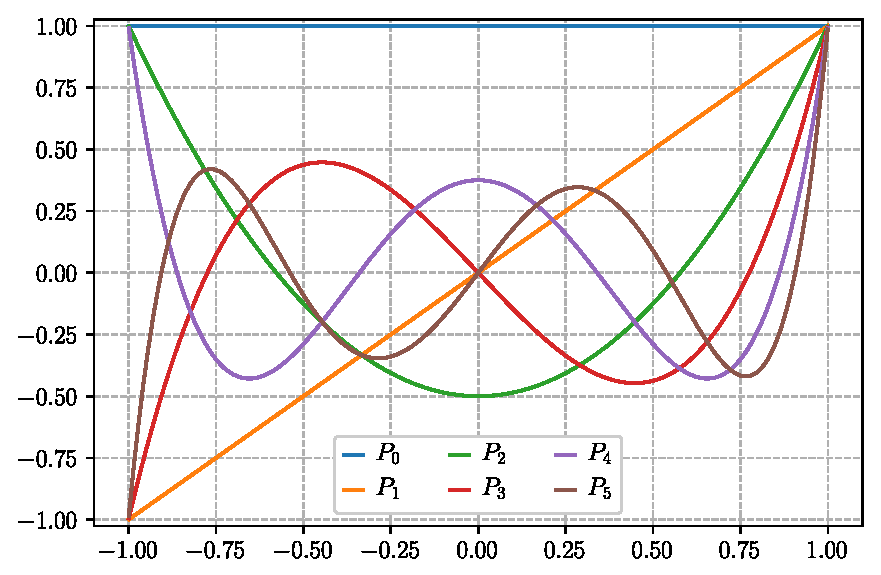
\includegraphics{figs/44b1338c42c47641d4f196cdfa949fe403e8df20.eps}
\caption{Legendre Polynomials upto order 5}
\end{figure}

\hypertarget{properties}{%
\subsubsection{Properties}\label{properties}}

\begin{itemize}
\item
  Orthogonality: The set of Legendre polynomials form an orthogonal
  family, that means: \begin{align}
  \int_{-1}^1 L_m(x)L_n(x) dx = \frac{2}{2n+1}\delta_{mn}.
  \end{align}
\item
  Completeness: Legendre polynomials are compelete. This means that the
  given piecewise continuous function \(f(x)\) with finitely many
  discontinuities in the interval {[}-1,1{]}, can be approximated by the
  following sum: \begin{align}
  f_n(x)=\sum_{l=0}^{n}a_lL_l(x),
  \end{align}
\end{itemize}

in which \(a_l\) is a coefficient and \(L_k(x)\) is the Legendre
polynomial of order \(k\), and \(f_n(x) \to f(x)\) as \(n \to \infty\).

The completeness property can be written in the following form:

\begin{align}
\sum_{l=0}^{\infty}\frac{2l+1}{2}L_l(x)L_l(y) = \delta(x-y).
\end{align}

Note \(x\), \(y\in [-1,1]\) and
\(\delta(x-y) = \frac{1}{2\pi}\int_{-\infty}^{\infty}e^{ip(x-y)}dp\).

\begin{itemize}
\tightlist
\item
  Bonnet's recursion formula: The Legendre polynomials can also be
  defined as the coefficients in a formal expansion in powers of \(t\)
  of the generating function:
\end{itemize}

\begin{align}
\frac{1}{\sqrt{1-2xt+t^2}} = \sum_{n=0}^{\infty}L_n(x)t^n.
%\label{ceq1}
\end{align}

By differentiating the generating function with respect to \(t\), the following is obtained:

\begin{align}
\frac{x-t}{\sqrt{1-2xt+t^2}} = (1-2xt+t^2)\sum_{n=0}^{\infty}nL_n(x)t^{n-1}.
%\label{ceq2}
\end{align}

By substituting the denominator of the L.H.S of the above equation with
the summation and rearranging the whole equation we get: \begin{align}
nL_n(x)t^{n-1} - (2n+1)xL_n(x)t^n + (1+n)L_n(x)t^{n+1} = 0.
\end{align}

Equating terms with identical powers of \(t\) we find:

\begin{align}
(1+n)L_{1+n}(x) - (2n+1)xL_n(x) + nL_{n-1}(x) = 0.
\end{align}

\begin{itemize}
\tightlist
\item
  Other properties

  \begin{itemize}
  \tightlist
  \item
    \((2n+1)L_n(𝑥)=L'_{n+1}(x)−L'_{n−1}(x)\);
  \item
    \(L_n(x)\) is even or odd if \(n\) is even or odd:
    \(L_{n}(-x)=(-1)^{n}L_{n}(x)\);
  \item
    \(L_n(1)=1\) , \(L_n(−1)=(−1)^n\)
  \end{itemize}
\end{itemize}

\hypertarget{lagrange-interpolation-polynomials-nodal-basis}{%
\subsection{Lagrange Interpolation Polynomials (Nodal
Basis)}\label{lagrange-interpolation-polynomials-nodal-basis}}

For a grid on \(\hat{\omega}\) with \(p+1\) nodes
\(\Xi_{P+1}:= {\xi_0,\cdots,\xi_p}\) the Lagrange interpolation
polynomial of a smooth function \(f(\xi)\) on \([-1,1]\) is defined as
follows: \begin{equation}
I_pf(\xi) = \sum_{i=0}^{p} f(\xi_{i})\pi_i(\xi)  \quad
\end{equation}

With the \(p+1\) polynomials forming the Lagrangian interpolation basis
being defined as: \begin{equation}
\pi_i(\xi)  = \prod_{\substack{j=0\\i \neq j}}^p \frac{\xi - \xi_i}{\xi_i - \xi_j}  \quad 0 \leq i,j \leq p
\end{equation}

\hypertarget{properties-1}{%
\subsubsection{Properties}\label{properties-1}}

\begin{itemize}
\item
  An interesting property of the Lagrangian polynomials is the fact
  that: \(\pi_i(x_j)=\delta_{ij}\).
\item
  If the Lagrange polynomials are applied in the Gauss-Lobatto-Legendre (GLL) points, it is also
  possible to define them as follows:
\end{itemize}

\begin{equation}
    \pi_j(\xi) = \frac{-1}{N(N+1)} \frac{(1-{\xi}^2)L_N'(\xi)}{(\xi-\xi_j)L_N(\xi_j)}  \quad 0 \leq j \leq N 
\end{equation}

In other words, Lagrange interpolation polynomials can be expressed in
terms of Legendre polynomials.

\begin{itemize}
\tightlist
\item
  Lagrange polynomials have \textbf{Local support}, which means that they
  are non-zero only in a specific space, i.e {[}-1,1{]} and vanish
  identically outside these boundaries.
\end{itemize}

\hypertarget{spectral-element-method-in-1d}{%
\section{Spectral Element Method in
1D}\label{spectral-element-method-in-1d}}

In Spectral Element Methods, the integration domain \(\Omega\) is
partitioned into intervals (elements). In one dimension, a partition of $(a,b) \in \Omega$ with $E$ elements, which is denoted by $\Delta{E}$, can be written as

\begin{equation}
    \Delta{E} : a=x_0<x_1< \cdots < x_E =b.
\end{equation}

A reference or parent element is also defined as
\(\hat{\Omega}:[-1 < \xi < 1]\). Particularly in this report, the points
\(\xi\) correspond to the \textbf{GLL} points. For
the convenience of numerical integration (GLL quadrature rule), we need to
map the element from physical domain to the reference domain
\(\hat{\Omega}\).

In 1D, a simple mapping that relates the upper boundary \(x^{e}_u\) and
the lower boundary \(x^{e}_l\) of element \(e\) with the reference
element is \begin{equation}
    x^{e}(\xi) = \frac{1-\xi}{2}x^{e}_l+ \frac{1+\xi}{2}x^{e}_u = \frac{1+\xi}{2}(x^{e}_u-x^{e}_l)+x^{e}_l,
\end{equation}

where (\(x^{e}_u-x^{e}_l\)) is the element size \(h\). Also, the inverse mapping can be defined as \begin{equation}
    \xi(x^{e}) = 2\frac{x^{e}-x^{e}_l}{h}-1.
\end{equation}

For illustration, the 1D spectral element mesh of order 5 with 1 element
in a domain \(\Omega:[0,2]\) looks as follow:

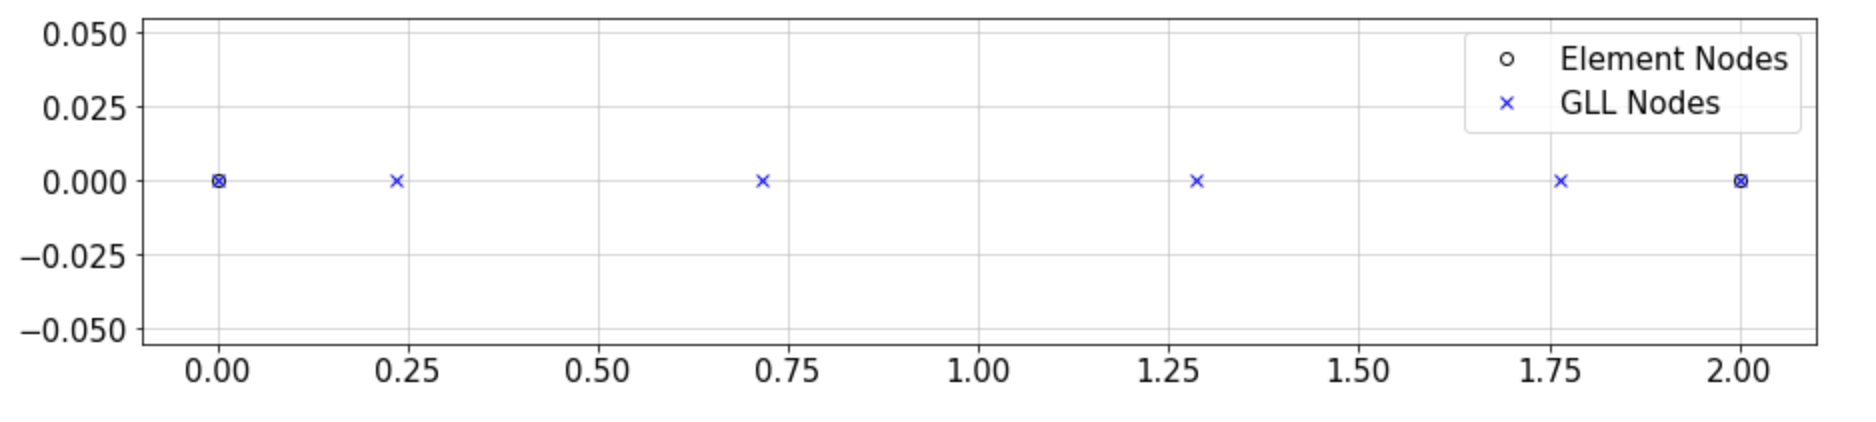
\includegraphics{figs/3bfea2e0211dfcbedca0466bd0dc58b20c68d586.png}

\hypertarget{continue-with-advectiondifussion.}{%
\subsection{Continue with
Advection-Difussion Equation}\label{continue-with-advectiondifussion.}}

Having chosen the GLL points for the reference grid, and by
choosing to follow a nodal approach, i.e.~chosen bases are the Lagrange
polynomials, it is possible to complete the discretization of the
advection-difussion equation: \begin{align}
\int_{\Omega} (v\frac{\partial u}{\partial t} + cv\frac{\partial u}{\partial x} + \nu\frac{\partial v}{\partial x}\frac{\partial u}{\partial x})dx = 0.
\end{align}

For this purpose, let us recall the process to derive the stiffness
matrix by only analizing the diffusion term and considering \(\nu=1\).
Starting from the following expresion: \begin{align}
\int_{\Omega^{e}} ( \frac{\partial v}{\partial x}\frac{\partial u}{\partial x})dx,
\end{align}

there are two main aspects to keep in mind:

\hypertarget{chain-rule}{%
\subsubsection{Chain Rule}\label{chain-rule}}

Considering the mapping, \(u\) and \(v\) can be expressed in the
following form: \begin{equation}
\left.u(x)\right\rvert_{\Omega^{e}}=\sum_{i=0}^{N}u_{i}^{e} \pi_{i}(\xi),  \quad \xi \in [-1,1].
\end{equation}

As such in the derivative of \(u\) with respect to \(x\) it is important
to consider the chain rule:

\begin{equation}
\left. \frac{\partial u(x)}{\partial x}\right\rvert_{\Omega^{e}}=\sum_{i=0}^{N} u_{i}^{e} \frac{\partial \pi_{i}}{\partial\xi}\frac{\partial\xi}{\partial x},  \quad \xi \in [-1,1].
\end{equation}

\hypertarget{change-of-integration-domain}{%
\subsubsection{Change of Integration
Domain}\label{change-of-integration-domain}}

Due to the mapping, the integration domain to evaluate the weak form
is changed. Consequently, the Jacobian determinant must be
introduced as a scaling factor, which for this case is:

\begin{equation}
J(\xi)=\frac{\partial x}{\partial \xi}=\frac{h}{2}.
\end{equation}

Introducing the previous notation into the diffusive term the following
is obtained:

\begin{equation}
\int_{\Omega^{e}} ( \frac{\partial v}{\partial x}\frac{\partial u}{\partial x})dx = \sum_{i=0}^{N}\sum_{j=0}^{N} v_i^{e}( \int_{\hat{\Omega}}\frac{\partial \pi_{i}}{\partial\xi}\frac{\partial \pi_{j}}{\partial\xi}(\frac{\partial\xi}{\partial x})^{2} J(\xi) d\xi)u_j^{e}.
\end{equation}

This yields a similar form as the one shown in the formulation of the
Galerkin method; however, additional terms that account for the mapping
and geometry of the element in physical domain are included now. For the
stiffness matrix in 1D, the geometry term becomes a constant since:

\begin{equation}
(\frac{\partial \xi}{\partial x})^{2} J(\xi)= (\frac{2}{h})^{2}\frac{h}{2}=\frac{2}{h}.
\end{equation}

Introducing the concepts into the original term produces:

\begin{equation}
\int_{\Omega^{e}} ( \frac{\partial v}{\partial x}\frac{\partial u}{\partial x})dx =(\underline{v}^{e})^{T}K^{e}\underline{u}^{e},
\end{equation}

where \begin{align}
K^{e}[i,j]&=\frac{2}{h}\int_{\hat{\Omega}}\frac{\partial \pi_{i}}{\partial\xi}\frac{\partial \pi_{j}}{\partial\xi} d\xi, \quad \hat{\Omega} \in [-1,1]. 
\end{align}

Up to the point, we have assumed that all integrals are evaluated
analytically. As we have seen, within each elemental domain we want to
evaluate integrals of the form \begin{equation}
\int_{-1}^{1}u(\xi) d\xi.
\end{equation} The form of \(u(\xi)\) is, however, problem specific and
therefore we need an automated way to evaluate such integrals. This
suggests the use of numerical integration or quadrature rule. The fundamental
concept is the approximation of the integral by a finite summation of
the form \begin{equation}
\int_{-1}^{1}u(\xi)d\xi = \sum_{i=0}^{Q-1}\rho_iu(\xi_i)+R(u),
\end{equation}

where \(\rho_i\) are specified constants or weights and \(\xi_i\)
represent an abscissa of \(Q\) distinct points in the interval
\(−1 \leq \xi_i \leq 1\). And \(R(u)\) is the residual. In particular,
we introduce Gauss-Lobatto-Legendre quadrature here: \begin{align}
    \xi_i &= 
    \begin{cases} 
      -1 & i= 0 \\
      \xi_{i-1,Q-2}^{1,1} & i=1,2... Q-2 \\
      1 & i = Q-1 
   \end{cases}\\
   \rho_i&=\frac{2}{N(N+1)}\frac{1}{[L_N(\xi_i)]^2}\\
   R(u) &= 0 ~~~~~\text{ if }~~~ u(\xi)\in\mathbf{P}_{2Q-3}([-1.1])
\end{align} In the above formulae \(L_Q(\xi)\) is the Legendre
polynomial. The zeros of the Jacobi polynomial \(\xi^{\alpha,\beta}\).
The GLL quadrature is accurate if the order of polynomial is no more
than \(2Q-3\). A better way to evaluate the zeros is the use of a
numerical algorithm such as a newton Rhapson technique. Having
determined the zeros, the weights can be evaluated from the formulae.
This is done by generating the Legendre polynomial from a recursion
relationship.

Then it is possible to numerically integrate and derivate the terms such
that the final form of the matrix is obtained:

\begin{align}
K^{e}[i,j]&=\frac{2}{h}\sum_{m=0}^{N} \rho_m D^{(1)}_{N,mi}D^{(1)}_{N,mj} 
\end{align}

Where \(D\) is the derivation matrix obtained as follows:

\begin{equation}
D_{N,ij}^{(1)} = \left. \frac{d\pi_j}{d\xi}\right\rvert_{\xi=\xi_i} =
     \begin{cases}
       \frac{L_N(\xi_i)}{L_N(\xi_j)}\frac{1}{\xi_i-\xi_j} &\quad\text{if }i \neq j \\
       -\frac{(N+1)N}{4} &\quad\text{if }i=j=0 \\
       \frac{(N+1)N}{4} &\quad\text{if }i=j=N \\
       0 &\quad\text{Otherwise } \\
     \end{cases}
\end{equation}

Following the same procedure as for the stiffness matrix, the mass and
convection matrices can also be obtained, keeing in mind that
\(\pi_i(x_j)=\delta_{ij}\): \begin{equation}
     M^{e}_{ij} := \frac{h}{2} \rho_i\delta_{ij} 
\end{equation}

\begin{align}
C^{e}[i,j]&=\sum_{m=0}^{N} \rho_m \pi_{mi}D^{(1)}_{N,mj}= \rho_iD^{(1)}_{N,ij} 
\end{align}

\hypertarget{extra-bit-what-about-non-linearities}{%
\paragraph{Extra bit: What about non
linearities?}\label{extra-bit-what-about-non-linearities}}

The non linear term in navier stokes equation and burger equation are
treated in a similar way as that of the constant convective term. For
the case where \(c=u(x)\). In this case, the same procedure is followed,
the bi-orthogonality of the basis functions used and taking advantage of
the quadrature rules, the following expression is obtained:
\begin{equation}
C^{e}_{N,ij}(u_i) =  \rho_i u_i^{e} D^{(1)}_{N,ij}
\end{equation}

Note that the convective matrix depends on \(u\) which needs to be taken
into consideration for time stepping. In a explicit method, the
Convective matrix would need to be evaluated each iteration.

\hypertarget{applying-boundary-conditions-homogenous-dirichlet-bc}{%
\subsubsection{Applying Boundary conditions: Homogenous Dirichlet
BC}\label{applying-boundary-conditions-homogenous-dirichlet-bc}}

\begin{itemize}
\item
  If \(u\in X_0^{N}\), the global (and local) basis coefficients on the
  boundary are zero: \begin{align}
  u_0 = u_0^1 = 0 \text{, and }u_{n+1} = u_N^E = 0
  \end{align}
\item
  And in our definition of global assemble matrix, the index is ranged
  from 0 to \(n\) on the global vectors \(v\) and \(u\).
\item
  Therefore we need to construct a restriction matrix \(R\) and
  prolongation matrix \(R^T\) that elimate \(u_0\) and \(u_{n+1}\). Note
  we can generate a matrix \(R^TR\) which can map function \(X^N\) to
  \(X^N_0\)
\end{itemize}

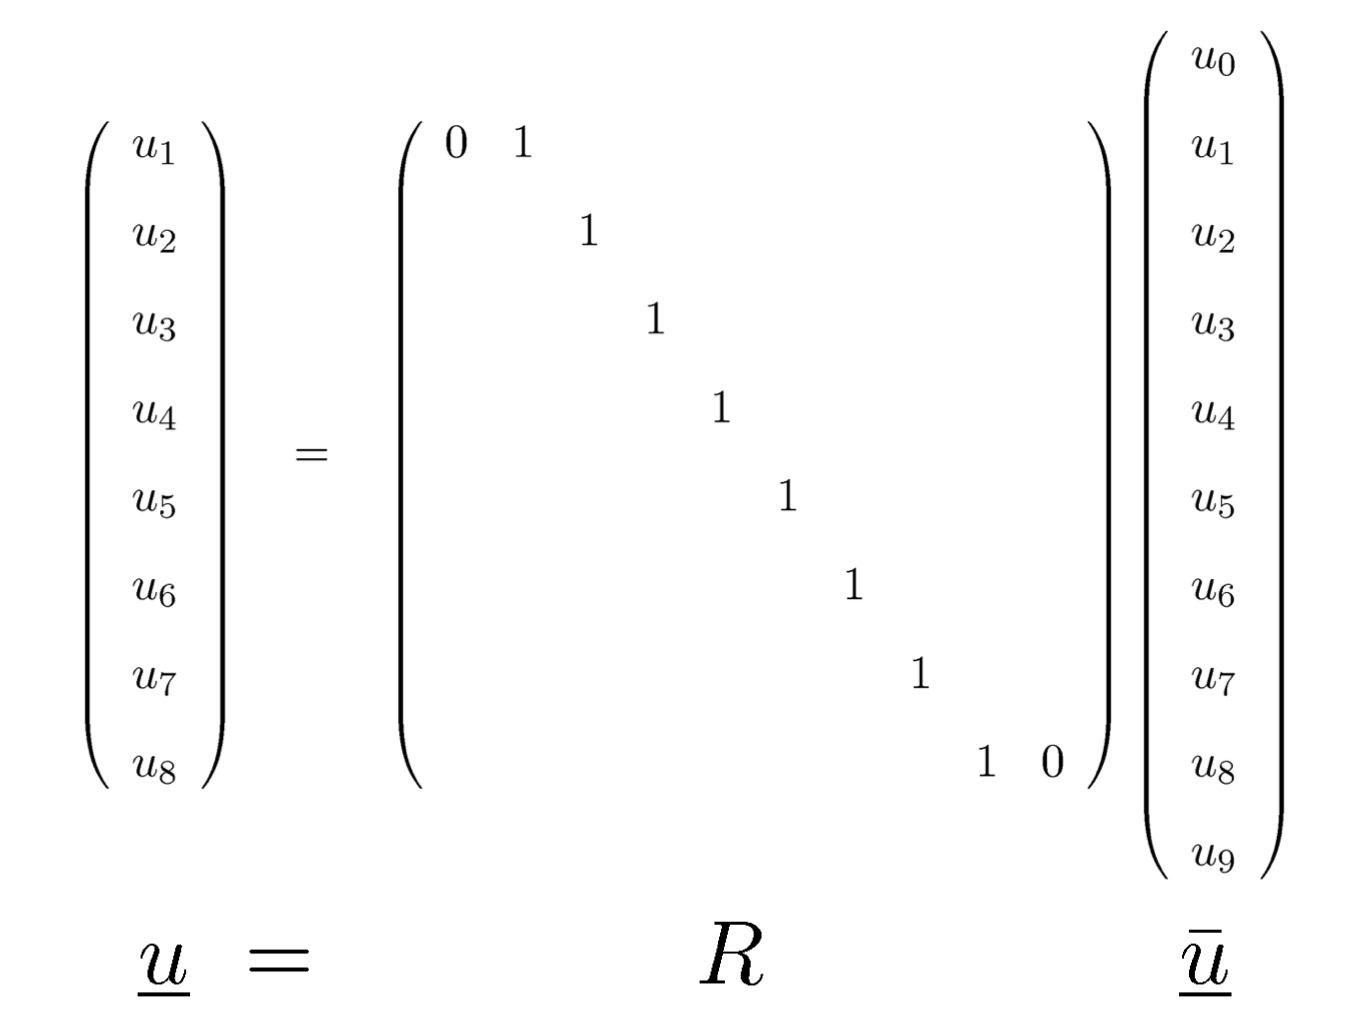
\includegraphics{figs/dadf8ccf703923cbac91fdb1eac78f62d729367f.png}
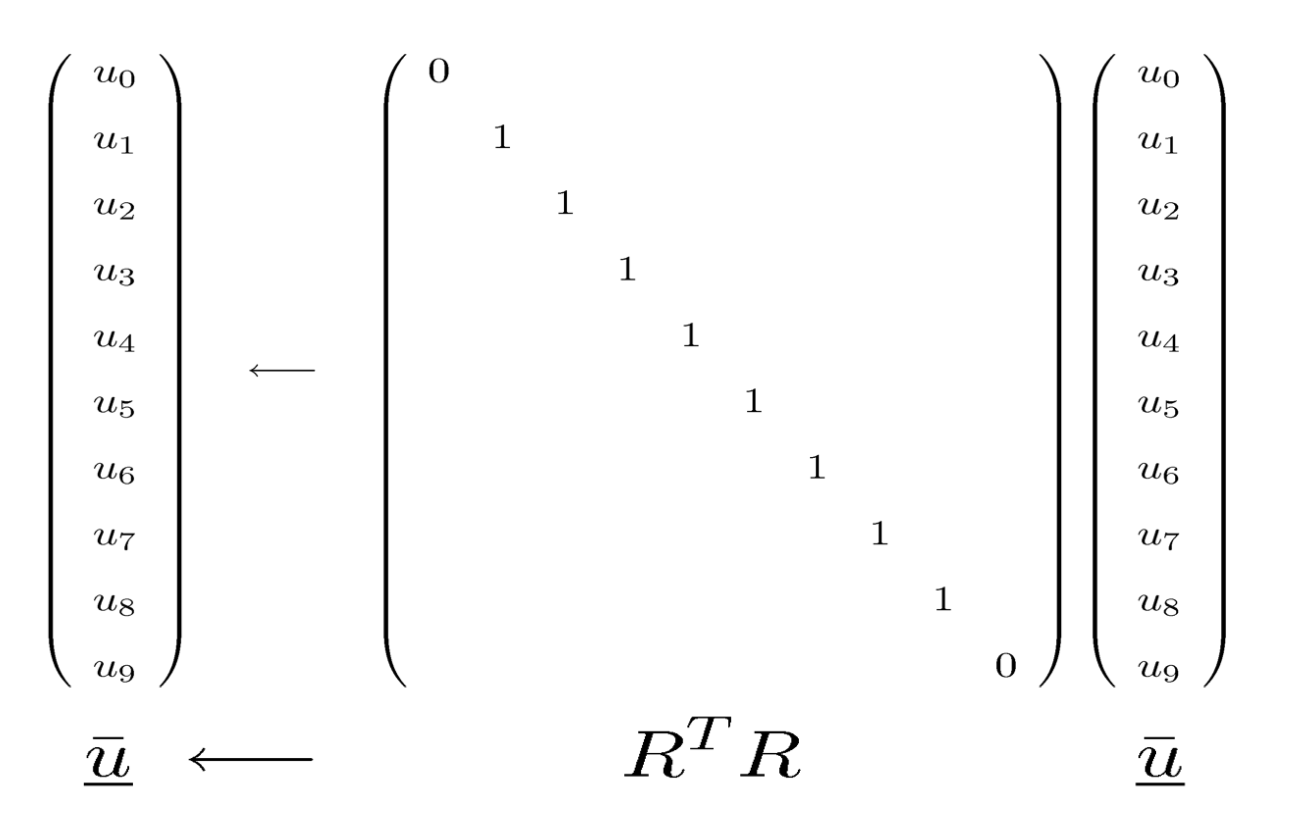
\includegraphics{figs/3c1003a64acccf7c33fd9604e81f9c4b75a66a3d.png}

\hypertarget{neumann-boundary-condition}{%
\subsubsection{Neumann boundary
condition}\label{neumann-boundary-condition}}

Let's Poisson equation as example for simplicity: \begin{align}
-\frac{d^2u}{dx^2} &= f(x)\\
u(-1) = 0&,u^{(1)}(1)=g
\end{align} Apply Galerkin method, integrate by part and apply Neumann
BC on the right boundary, Dirichlet BC on the left boundary:
\begin{equation}
\int_{-1}^1\frac{dv}{dx}\frac{du}{dx}dx = \int_{-1}^1 vf(x)dx+v(1)g
\end{equation} We can see only the last equation is modified. We can
continue with the direvation and reach to the linear system:
\begin{equation}
Au=F
\end{equation}

Rewrite it into the matrix format:

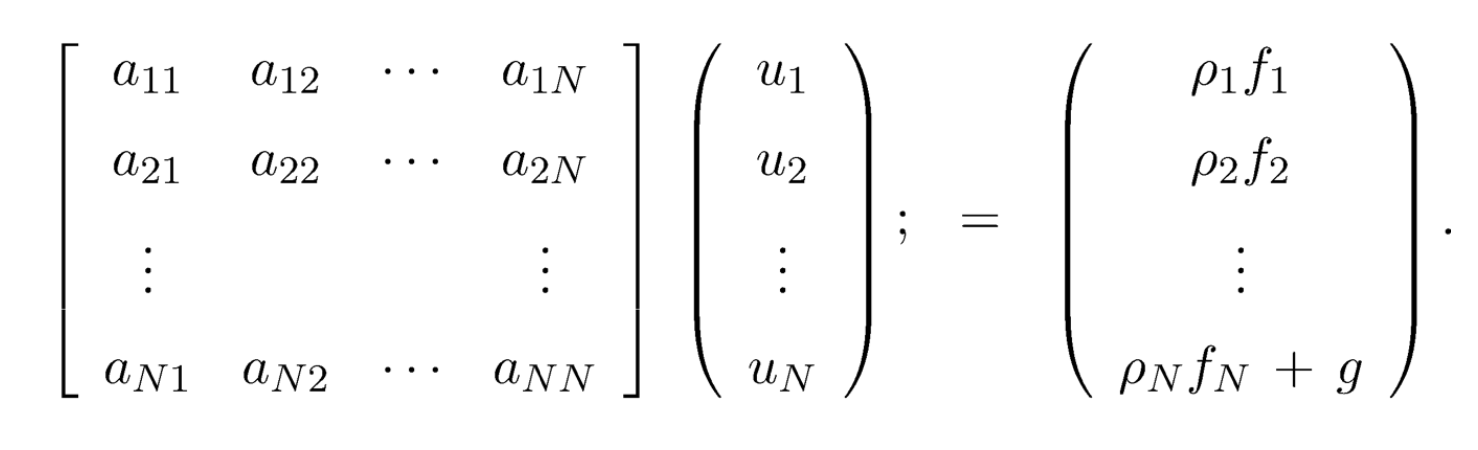
\includegraphics{figs/ee2417c98a1e9e26931e69be51638abdfd2367c9.png}

We can see only the last term in the forcing vector is modified due to
the Neumann BC.

\hypertarget{time-integration}{%
\subsubsection{Time integration}\label{time-integration}}

We have linear system: \begin{align}
u_t = \lambda u
\end{align} where \(\lambda\in\mathbb{C}\) is a system parameter which
mimics the eigenvalues of linear systems of differential equations.

The equation is stable if Real(\(\lambda\)) \(\leq 0\). In this case the
solution is exponentially decaying. (\(lim_{t\to\infty}u(t) = 0\)).

Explicit Euler method: \begin{align}
u^{n+1} &= u^{n} + h\lambda u^{n}
=(1+h\lambda)u^{n}
=(1+h\lambda)^{n+1}u^0
\end{align}

Where \(h=\Delta t\). So for explicit Eular method, if we want solution
to be stable as \(t\to\infty\), \(|1+\lambda h|<1\). In the complex
plane, we can find the optimal \(h\) by making every \(\lambda h\)
inside the neutral stability curve.

\begin{figure}
\centering
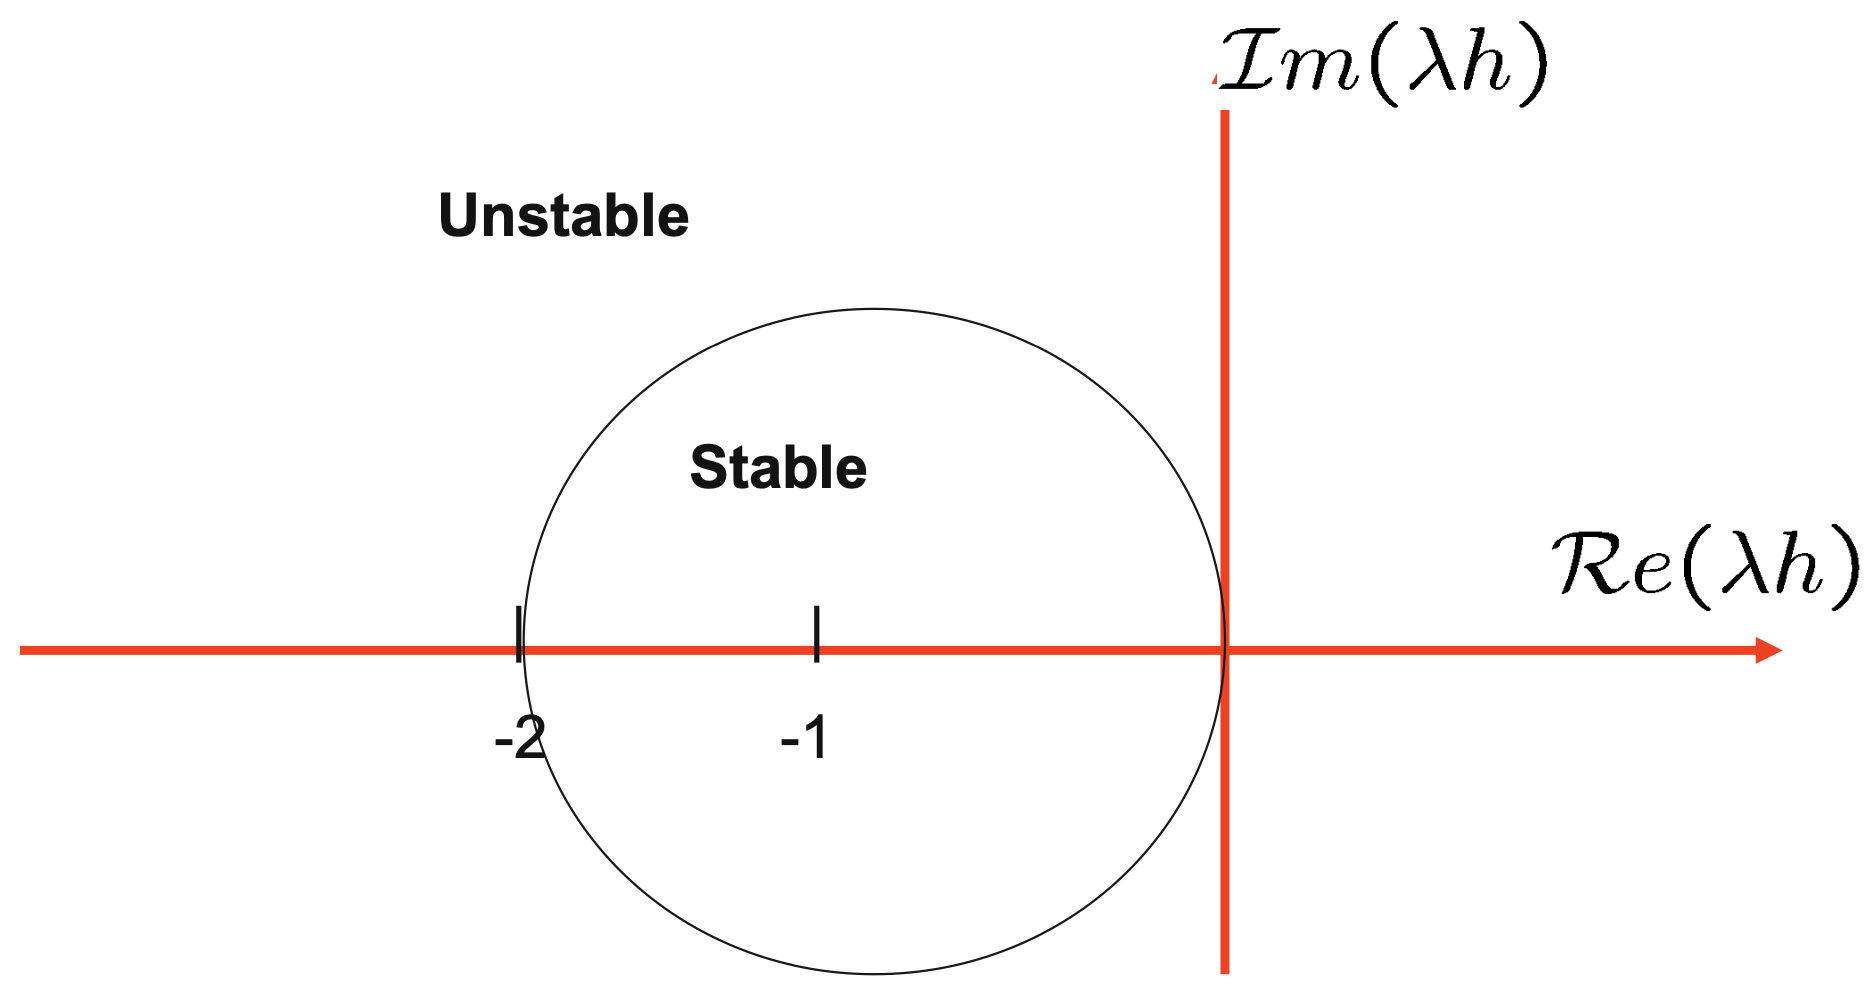
\includegraphics{figs/0d2289a81eb4c5c10c4430bc8fdffb2cc397e0ba.png}
\caption{stability\textbar20\%}
\end{figure}

The final result with \(p=32, t=0.1\) and Dirichlet BC on both sides
comparing with the initial condition:

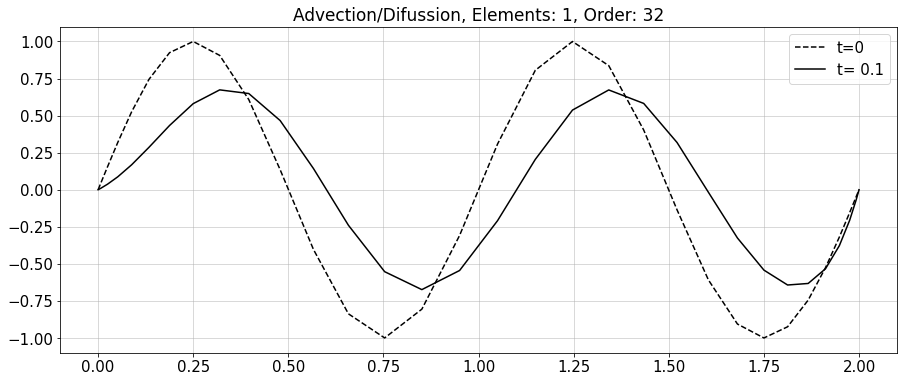
\includegraphics{figs/3d969364028d7ae5e24eb792b401314b71724e68.png}

\hypertarget{relationship-between-modal-and-nodal-basis}{%
\subsection{Relationship between Modal and Nodal
Basis}\label{relationship-between-modal-and-nodal-basis}}

The key historical distinction between a spectral element and a p-type
finite element is whether the expansion is nodal or modal. As has been
mentioned previously the Galerkin approximation is the minimising
solution independent of the polynomial approach so if there are no
integration errors then the methods are mathematically equivalent.
However each approach does have different numerical properties in terms
of efficiency of implementation, ability to vary the polynomial order
and the conditioning of the global matrix systems.

\hypertarget{nodal-approach}{%
\subsubsection{Nodal approach}\label{nodal-approach}}

Till now, we used the Lagerange interpolations at GLL points to build
our trail function. The elemental mass matrix using this expansion is
full if we evaluate the inner product \(M[p][q] = (\pi_p,\pi_q)\)
exactly. If, however, we use the Gauss-Legendre-Lobatto quadrature rule
corresponding to the same choice of nodal points on which the expansion
was defined, the mass matrix is diagonal due to the Kronecker delta
property: \begin{equation}
M[p][q] = (\pi_p,\pi_q) \approx\sum_{i=0}^{Q}\rho_i\pi_p(\xi_i)\pi_q(\xi_i) = \sum_{i=0}^{Q}\rho_i\delta_{pi}\delta_{qi} = \rho_p\delta_{pq}
\end{equation} where \(\rho_i\) are the weights for the
Gauss-Legendre-Lobatto rule using \(Q+1\) points. The quadrature rule
using \(Q + 1\) points is exact only for polynomials of order \(2Q-3\).
The diagonal components of the elemental mass matrix using the
reduced-order quadrature rule are equal to the row sum of the elemental
mass matrix using exact integration. Summing the rows and using this as
the entry of a diagonal matrix is common practice in finite elements and
is known as lumping the mass matrix. In the standard finite element
case, lumping the mass matrix is an approximation, but in the spectral
element case this lumping has a direct equivalence. \begin{equation}
\sum_{q=0}^Q M[p][q] = \sum_{q=0}^Q(\pi_p,\pi_q) =(\pi_p(\xi),\sum_{q=0}^Q\pi_q(\xi))
\end{equation} We note that the sum of the Lagrange basis over all modes
is simply `1': \(\sum_{q=0}^Q\pi_q(\xi)=1\), and so the sum of the pth
row becomes: \begin{equation}
\sum_{q=0}^Q M[p][q]  =(\pi_p(\xi),\sum_{q=0}^Q\pi_q(\xi))= (\pi_p(\xi),1)
\end{equation} The last term here we call it, as defination, weight
corresponding to the \(p^{th}\) point in the Gauss-Lobatto-Legendre
quadrature rule using \(Q\) points.

As a final point, we note that the elemental Laplacian matrix using the
spectral element expansion does not have any notable properties of this
type and is full for all choices of quadrature order.

\hypertarget{modal-approach}{%
\subsubsection{Modal approach}\label{modal-approach}}

Thanks to the orthogonality of Legendre polynomail: \begin{align}
\int_{-1}^1 P_m(x)P_n(x) dx = \frac{2}{2n+1}\delta_{mn} 
\end{align} we can construct the elemental mass matrix easily using this
relationship. Worth to note that more generally, the sequence of
polynomial functions \({\{p_k\}}^{\infty}_{k=0}\), where the degree of
\(p_k\) is equal to \(k\), forms a system of orthogonal polynomials with
respect to \(\omega\) if: \begin{equation}
(p_k,p_l)_{L_w^2}:=\int_{-1}^1\omega(x)p_k(x)p_l(x)dx= \gamma_k\delta_{kl}
\end{equation} where \(L_w^2\) is the Hilbert space of
Lebesgue-weighted-square-integrable functions and \(\omega\) denote any
nonnegative integrable weight function. \(\gamma_k:=\|p_k\|^2_{L_w^2}\).

Now, we can plot the structure of mass matricex via different
approaches:

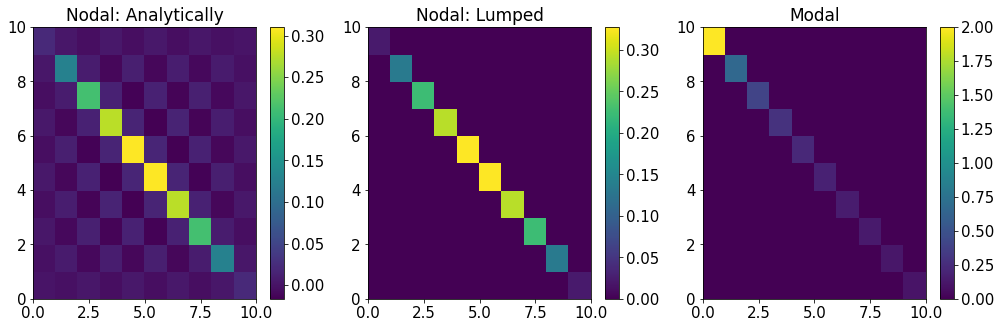
\includegraphics{figs/64cf6104567524d8214da8aaba5fa3b1b72eea69.png}

\hypertarget{spectral-element-method-in-1d---multiple-elements}{%
\section{Spectral Element Method in 1D - Multiple
Elements}\label{spectral-element-method-in-1d---multiple-elements}}

The subdivision of the physical domain \(\Omega\) into multiple elements
has been stated, but the practical application of it has not. To start,
it is very important to analize continuity between the elements.

\hypertarget{continuity-scatter-gather}{%
\subsection{Continuity
(Scatter-Gather)}\label{continuity-scatter-gather}}

One of the advantages of using Lagrangian basis in SEM is the fact that
function continuity is enforced by equating coincident nodal values,
that is: \begin{equation}
    x_{i}^{e}=x_{\hat{i}}^{\hat{e}} => u_{i}^{e}=u_{\hat{i}}^{\hat{e}}
\end{equation}

Defining \(\mathcal{N}\) as the number of distinct nodes in \(\Omega\),
the previous equation represents \((N+1)^{d}E-\mathcal{N}\) constrains
on the choice of local nodal value \(u_{i}^{e}\).

The constrain can be recasted in matrix from, Keeping in mind that the
global nodal values can be represented in vector form \(\underline{u}\)
as well as the local element wise nodal values \(\underline{u}^{e}\). If
a collection of element nodal values is defined as a collection of local
vectors \(\underline{u}_L\) such that:

\begin{equation}
    \underline{u}_L=
    \begin{pmatrix}
    \underline{u}^{1} \\
    \underline{u}^{2} \\
    \cdots \\
    \underline{u}^{e} \\
    \cdots \\
    \underline{u}^{E} \\
    \end{pmatrix}= 
    \begin{pmatrix}
    {u}^{1}_{0} \\
    {u}^{1}_{1} \\
    \cdots \\
    {u}^{e}_{0} \\
    {u}^{e}_{1} \\
    \cdots \\
    {u}^{E}_{N} \\
    \end{pmatrix}
\end{equation}

If \(u\) is continous, then there exist a boolean contectivity matrix
\(Q\) that maps \(\underline{u}\) to \(\underline{u}_L\) ensuring that
the constrains are satisfied. Such that: \begin{equation}
    \underline{u}_L=Q\underline{u}
\end{equation}

The matrix \(Q\) is known as the \textbf{Scatter} operator and its
action is to \textbf{copy} entries from the global domain into the local
one.

An aditional matrix \(Q^{T}\) is also defined, which is known as the
\textbf{Gather} operator: \begin{equation}
    \underline{v}=Q^{T}\underline{u}_L
\end{equation}

The function of this operation is to \textbf{sum entries} from
corresponding nodes, which is why \(\underline{v} \neq \underline{u}\)

For instance, the shape of \(Q\) in 1D for 2 elements and a basis of
order 1 is as follows: \begin{equation}
    Q=
    \begin{pmatrix}
           1    &   0     &0 \\
           0    &    1    & 0\\
            0  &   1     & 0\\
            0   &    0    & 1
    \end{pmatrix} 
\end{equation}

Thus, \(\underline{u}_L\) for this case is as follows:

\begin{equation}
    \underline{u}_L=
    \begin{pmatrix}
    {u}^{1}_{0} \\
    {u}^{1}_{1} \\
    {u}^{2}_{0} \\
    {u}^{2}_{1} \\
    \end{pmatrix}=
    \begin{pmatrix}
    {u}_{0} \\
    {u}_{1} \\
    {u}_{1} \\
    {u}_{2} \\
    \end{pmatrix}=
     \begin{pmatrix}
           1    &   0     &0 \\
           0    &    1    & 0\\
            0  &   1     & 0\\
            0   &    0    & 1
    \end{pmatrix} 
    \begin{pmatrix}
    {u}_{0} \\
    {u}_{1} \\
    {u}_{2} \\
    \end{pmatrix}=
    Q\underline{u}
\end{equation} It is clear that using the scatter operator, the values
from the global matrix are copied to the local ones. For example, the
global value \({u}_{1}\), which is the value of the common grid between
elemets 1 and 2, is coppied to local coefficients \({u}^{1}_{1}\) and
\({u}^{2}_{0}\).

A gather-scatter operation can be defined such that \(\Sigma'=QQ^{T}\)
which is denoted as \textbf{Direct Stiffness Summation} which is a local
to local transformation that amounts to summing shared interface
variables and redistributing them to their original locations, leaving
the interior nodes unchanged.

\textbf{Note:} In practice, the matrices \(Q\) and \(Q^T\) are never
constructed. Rather, their actions are implemented using indirect
addressing.

\hypertarget{construction-of-a-global-basis}{%
\subsection{Construction of a Global
Basis}\label{construction-of-a-global-basis}}

Once again, for simplicity the process will be initially shown for the
diffusion term. It has been stated that for a given element, the
following is true:

\begin{equation}
\int_{\Omega^{e}} ( \frac{\partial v}{\partial x}\frac{\partial u}{\partial x})dx =(\underline{v}^{e})^{T}K^{e}\underline{u}^{e}
\end{equation}

The extension of this expression to the whole domain is the following:
\begin{equation}
    \int_{\Omega} ( \frac{\partial v}{\partial x}\frac{\partial u}{\partial x})dx = \sum_{e=1}^{E} (\underline{v}^{e})^{T}K^{e}\underline{u}^{e} = (\underline{v}_L)^{T}K_L\underline{u}_L    
\end{equation}

Where \(\underline{u}_L\) and \(\underline{v}_L\) have already been
defined and \(K_L\) is defined as the \textbf{Unassembled Stiffness
Matrix}, which has the next form:

\begin{equation}
        K_L=
        \begin{pmatrix}
        K^1 &           &        & \\
                  & K^2 &        & \\
                  &           & \cdots & \\
                  &           &        & K^{E}
        \end{pmatrix} 
\end{equation}

Since the previous finding holds for continous \(u,v\), based on the
discussion on previous sections, it is possible to say that there exist
boolean matrices and vectors \(\underline{u}, \underline{v}\) such that
\(\underline{u}_L=Q\underline{u}\) and
\(\underline{v}_L=Q\underline{v}\).

Applying this knowledge into the system yields:

\begin{equation}
        \int_{\Omega} (\nabla u \nabla v) \,d\textbf{x} = (\underline{v})^{T}Q^{T}K_LQ\underline{u}    
\end{equation}

Where \(K=Q^{T}K_LQ\) is known as the \textbf{Assmebled Stiffness
Matrix}.

Following the same reasoning, it is also possible to find an expression
for the other matrices: \begin{equation}
M = Q^{T}M_LQ    
\end{equation}

\begin{equation}
C = Q^{T}C_LQ    
\end{equation}

The problem is then solved in the global domain as follows:
\begin{equation}
M\frac{d\underline{u}}{dt}=-K\underline{u}-C\underline{u}
\end{equation}

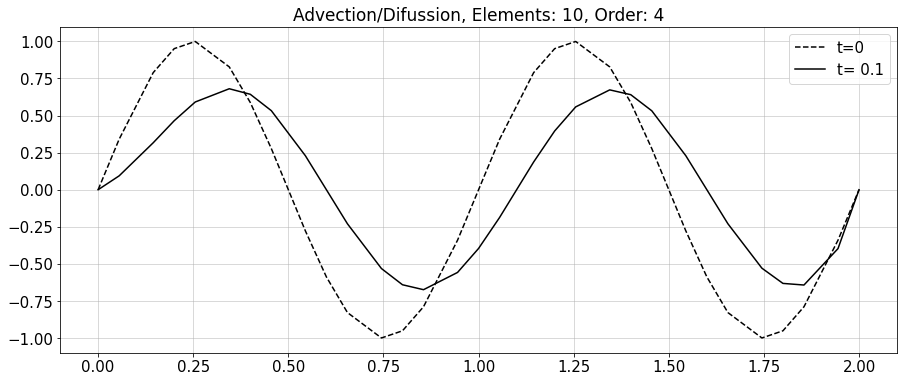
\includegraphics{figs/da09c33b2e35ea401b49fefd07523c278274758d.png}

\hypertarget{note-of-caution---discontinous-terms.}{%
\subsubsection{Note of Caution - Discontinous
terms.}\label{note-of-caution---discontinous-terms.}}

The use of \(Q\) to map from local to global is restricted to continous
functions. If in the original equation we had a source term \(f\) such
that:

\begin{equation}
\frac{\partial{u}}{\partial{t}} + c \frac{\partial{u}}{\partial{x}} =  \nu \frac{\partial^{2}u}{\partial{x}^{2}}+f
\end{equation}

An aditional term to discretize would have the next form:

\begin{equation}
        \int_{\Omega} (v f) \,d\textbf{x}        
\end{equation}

Performing the same procedure as done with the other terms, i.e express
\(f\) as \(f(\textbf{x})=\sum_{i=0}^{N}f_{i} \pi_{i}(\xi)\), construct
element matrix and then generalize. Will yield the next results:

\begin{equation}
        \int_{\Omega} (v f) \,d\textbf{x} = (\underline{v})^{T}Q^{T}M_L\underline{f}_L        
\end{equation}

Where for this case, the expression \(\underline{f}_L=Q\underline{f}\)
can not be applied a priori since the source terms might be discontinous
across boundaries.

\hypertarget{working-in-local-terms}{%
\subsubsection{Working in Local terms}\label{working-in-local-terms}}

Another way to express the formulation: \begin{equation}
         Q^{T}M_{L}Q\frac{d\underline{u}}{dt} = - Q^{T}K_LQ\underline{u} - Q^{T}C_LQ\underline{u}    
\end{equation} Multiplying the Global formulation by \(Q\) yields:
\begin{equation}
         \Sigma' M_{L}\frac{d\underline{u}_{L}}{dt} = - \Sigma'K_L\underline{u}_L - \Sigma'C_L\underline{u}_L    
\end{equation}

From this new formulation certain aspects are gained. It is now possible
to work on each element localy, evaluating operations without the need
to map from gobal to local terms. Adittionally, the gatter and scatter
operations are now done in sequence, which for paralell processes
reduces the overhead produced due to data communication.

\hypertarget{spectral-element-method---multiple-dimensions}{%
\section{Spectral Element Method - Multiple
Dimensions}\label{spectral-element-method---multiple-dimensions}}

For the extension of the formulation to multiple dimensions is it
beneficial to explain some concepts first.

\hypertarget{definition-tensor-product}{%
\subsection{Definition: Tensor
Product}\label{definition-tensor-product}}

Let \(A\) and \(B\) be \(k\) x \(l\) and \(m\) x \(n\) matrices. A
\(km\) x \(ln\) matrix \(C\) of the next form can be defined:
\begin{equation}
C=
\begin{pmatrix}
a_{11}B & a_{12}B & \cdots & a_{1l}B\\
a_{21}B & a_{22}B & \cdots & a_{2l}B\\
\cdots & \cdots & \cdots & \cdots\\
a_{k1}B & a_{k2}B & \cdots & a_{kl}B
\end{pmatrix}
\end{equation}

For this case, \(C\) is said to be the tensor product of \(A\) and \(B\)
and can be denoted as:

\begin{equation}
    C=A \otimes B
\end{equation}

The definition of tensor product is very important, as many operations
in the multidimensional problems using SEM end up acquiring this form,
and using tensor products allows for simplifications on the application
of linear operators to the quantities.

\hypertarget{definition-matrix-free-formulation---explained-in-2d}{%
\subsection{Definition: Matrix Free Formulation - Explained in
2D}\label{definition-matrix-free-formulation---explained-in-2d}}

Consider the next representation of \(u\) in the reference
domain\((x,y) \in \hat{\Omega}:=[-1,1]^{2}\)

\begin{equation}
    u(x,y)=\sum_{i=0}^{M}\sum_{j=0}^{N} u_{ij} \pi_{M,i}(x) \pi_{N,j}(y) 
\end{equation}

It is possible to use a \textbf{vector representation} of the
coefficients as follows:

\begin{equation}
    \underline{u} := (u_1,u_2,\cdots,u_l,\cdots,u_{\mathcal{N}})^{T}=(u_{00},u_{10},\cdots,u_{IJ},\cdots,u_{MN})^{T} 
\end{equation}

where \(\mathcal{N}=(M+1)(N+1)\) is the number of basis coeficcients and
the mapping \(l=1+i+(M+1)j\) translates the two-index coefficient
representation to standard vector form , with the leading coefficient
advancing more rapidly.

The derivative with respect to \(x\) of \(u(x,y)\) at the GLL points is:
\begin{equation}
    w_{pq}=\frac{\partial u}{\partial x}_{\xi_{M,p},\xi_{N,q}}=\sum_{i=1}^{M}\sum_{j=1}^{N} u_{ij} \pi_{M,i}'(\xi_{M,p}) \pi_{N,j}(\xi_{N,q})= \sum_{i=1}^{M} u_{iq} \pi_{M,i}'(\xi_{M,p})
\end{equation}

Can be represented in matrix-vector product form as shown here:
\begin{equation}
    \underline{w}=D_x\underline{u}=
    \begin{pmatrix}
    \hat{D}_x &           &        & \\
              & \hat{D}_x &        & \\
              &           & \cdots & \\
              &           &        & \hat{D}_x
    \end{pmatrix} 
    \begin{pmatrix}
    u_{00} \\
    u_{10} \\
    \cdots \\
    u_{MN}
    \end{pmatrix}
\end{equation}

Where \(\hat{D}_x\) is the one dimensional derivative matrix associated
with the GLL points and which is applied to each row of the coefficients
matrix. The \(y\) derivative would be then defined following a similar
process but applying the matrix \(\hat{D}_y\) to each column. The
general derivative operators can be defined very easily by using the
tensor product definitions, which yields: \begin{equation}
    D_x=I \otimes \hat{D}_x \quad  D_y= \hat{D}_y \otimes I
\end{equation}

In the evaluation of multidimentional PDE, matrix-vector multiplications
of the form \(\underline{v}=(A \otimes B)\underline{u}\) are very common
and normaly defined as: \begin{equation}
    v_{ij}=\sum_{l=1}^{n}\sum_{k=1}^{m} a_{jl} b_{ik} u_{kl} \quad i=1,\cdots,m \quad j=1,\cdots,n
\end{equation}

In vector form, and thanks to the associativity of tensor product, the
same expression can be recast as follows: \begin{equation}
    C\underline{u}=(A \otimes I)(I \otimes B)\underline{u}
\end{equation}

In practice, however, the matrix \(C\) does not need to be formed, as
one can evaluate the effect of matrix \(C\) on the vector as follows:

\begin{itemize}
\tightlist
\item
  Compute \(\underline{w}=(I \otimes B)\underline{u}\) \begin{equation}
        w_{ij}=\sum_{k=1}^{m} b_{ik} u_{kj} \quad i=1,\cdots,m \quad j=1,\cdots,n
  \end{equation}
\item
  Then compute \(\underline{v}=(A \otimes I)\underline{w}\)
  \begin{equation}
        v_{ij}=\sum_{l=1}^{m} a_{jl} w_{il}  = \sum_{l=1}^{m} w_{il} a_{lj}^{T}  \quad i=1,\cdots,m \quad j=1,\cdots,n
  \end{equation}
\end{itemize}

This way, the evaluations can be done with a lower number of operations.

\hypertarget{matrix-matrix-operators}{%
\subsubsection{Matrix-Matrix Operators}\label{matrix-matrix-operators}}

It is important to note that if the vector \(\underline{u}\) is viewed
as a matrix \(U\) such that \(\{U\}_{ij}=u_{ij}\), then the tensor
products can be recasted in the following form: \begin{equation}
        (A \otimes B)\underline{u} = BUA^{T}
    \end{equation}

These properties are extremely benefical to the performance of Spectral
Element solvers.

\hypertarget{getting-the-element-operators}{%
\subsection{Getting the Element
Operators}\label{getting-the-element-operators}}

The are many similarities with the process to get the element operators
in 1D to extended dimensions.

Note that in the spectral element method, each element on the physical
domain \(\textbf{x} \in \Omega\) must be mapped to the reference element
in the computational domain \(\textbf{r} \in \hat{\Omega}\)

Usually isoparametric mappings are employed as the following one in 2D:
\begin{equation}
\left.x(r,s)\right\rvert_{\Omega^{e}}=\sum_{i=0}^{N}\sum_{j=0}^{N} x_{ij}^{e} \pi_{i}(r) \pi_{j}(s) \quad (r,s) \in (-1,1)^{2}
\end{equation}

The representation of a variable in physical domain is then expressed as
a function of lagrange interpolants that vary in the computational
domain, as in the next example in 2D: \begin{equation}
    u(x,y)=\sum_{i=0}^{M}\sum_{j=0}^{N} u_{ij} \pi_{M,i}(r) \pi_{N,j}(s) 
\end{equation}

Equal care must be taken with certain aspects, just as in the one
dimentional SEM.

\hypertarget{chain-rule-1}{%
\subsubsection{Chain Rule}\label{chain-rule-1}}

Derivative taken with respect to variables in the original domain must
take into consideration the chain rule: \begin{equation}
    \frac{\partial u}{\partial x}=\frac{\partial u}{\partial r}\frac{\partial r}{\partial x}+\frac{\partial u}{\partial s}\frac{\partial s}{\partial x} 
\end{equation}

or in \(\mathcal{R}^{d}\): \begin{equation}
    \frac{\partial u}{\partial x_k}=\sum_{k=1}^{d}\frac{\partial u}{\partial r_i}\frac{\partial r_i}{\partial x_k}
\end{equation}

\hypertarget{change-of-integration-domain-1}{%
\subsubsection{Change of Integration
Domain}\label{change-of-integration-domain-1}}

Changing the integration domain, from the physical to the reference,
brings with itself the necesity to include the appropiate scaling
factor. Thus, it is needed to recall the definition of the
\textbf{Jacobian Determinant}:

\begin{equation}
    J(\textbf{r})=\det\frac{\partial x_i}{\partial r_j}=det
    \begin{pmatrix}
    \frac{\partial x_1}{\partial r_1} & \cdots & \frac{\partial x_1}{\partial r_d}\\
    \cdots & \cdots & \cdots\\
    \frac{\partial x_d}{\partial r_1} & \cdots & \frac{\partial x_d}{\partial r_d}\\
\end{pmatrix}
\end{equation}

Keeping in mind these definitions, the discratization of the diffusive
term is presented in order to ilustrate the process. The d dimentional
form of the bilinear diffusive term for a given element is the
following:

\begin{equation}
    \mathcal{A}(v,u)=\sum_{k=1}^{d} \int_{\Omega^{e}} \frac{\partial v}{\partial x_k}\frac{\partial u}{\partial x_k} d\textbf{x} 
\end{equation}

The chain rule is applied on the derivatives and a change of variable is
done in the integration domain from \(\Omega^{e}\) to \(\hat{\Omega}\):
\begin{equation}
    \mathcal{A}(v,u)=\sum_{i=1}^{d} \sum_{j=1}^{d} \int_{\hat{\Omega}} \frac{\partial v}{\partial r_i} (\sum_{k=1}^{d}\frac{\partial r_i}{\partial x_k}\frac{\partial r_j}{\partial x_k} J(\textbf{r})) \frac{\partial u}{\partial r_j} d\textbf{r} 
\end{equation}

Following this, all the metrics and geometry asociated variables can be
grouped together into a variable:

\begin{equation}
\mathcal{G}_{ij}(\textbf{r})=\sum_{k=1}^{d}\frac{\partial r_i}{\partial x_k}\frac{\partial r_j}{\partial x_k} J(\textbf{r}) \quad 1 \leq i,j \leq d
\end{equation}

The integrals in the difussion term can be numerically treated thanks to
the quadrature rule, such that the following is obtained:

\begin{equation}
    \mathcal{A}(v,u)=\sum_{i=1}^{d} \sum_{j=1}^{d} \sum_{klm}^{N} \left[ \frac{\partial v}{\partial r_i}  \mathcal{G}_{ij}(\textbf{r}) \frac{\partial u}{\partial r_j} \right]_{(\xi_k,\xi_l,\xi_m)} \rho_k \rho_l \rho_m 
\end{equation}

All that is left is to represent \(u\) and \(v\) as a basis and
coefficients in terms of the lagrangian polynomials. In this case, the
differentiation procedures follows similar to the one already shown. The
example for one derivative is the following:

\begin{equation}
    \frac{\partial u}{\partial r_1}\rvert_{(\xi_k,\xi_l,\xi_m)}=\sum_{p=0}^{N} \hat{D}_{kp}u_{plm}= (I \otimes I \otimes \hat{D})\underline{u}, \quad k,l,m \in \{0, \cdots, N\}^{3}
\end{equation}

Grouping the geometric terms and quadrature weights into a set of
\(d^2\) diagonal matrices \(G_{ij}, i,j \in {1,\cdots, d^2}\) such that:

\begin{equation}
    (G_{ij})_{\hat{k}\hat{k}}=\left[ \mathcal{G}_{ij}  \right]_{(\xi_k,\xi_l,\xi_m)} \rho_k \rho_l \rho_m
\end{equation}

with \(\hat{k}=1+k+(N+1)l+(N+1)^{2}m\);
\(k,l,m \in \{0, \cdots, N \}^{3}\)and defining: \begin{equation}
    D_1=(I \otimes I \otimes \hat{D}) \quad D_2=(I \otimes \hat{D} \otimes I) \quad D_3=(\hat{D} \otimes I \otimes I)
\end{equation}

It is possible to combine all the operators to achieve one compact form
of the energy inner product:

\begin{equation}
    \mathcal{A}(v,u)= \underline{v}^{T}
    \begin{pmatrix}
    D_1 \\
    D_2 \\
    D_3 \\
    \end{pmatrix}^{T} 
    \begin{pmatrix}
    G_{11} & G_{12} & G_{13}\\
    G_{21} & G_{22} & G_{23}\\
    G_{31} & G_{23} & G_{33}\\
    \end{pmatrix} 
    \begin{pmatrix}
    D_1 \\
    D_2 \\
    D_3 \\
    \end{pmatrix} \underline{u}=\underline{v}^{T}D^{t}GD\underline{u}
\end{equation}

From this expression, the element stiffness matrix is defined as
\(K^{e}=D^{T}GD\).

The Mass matrix is obtained by an extension of the previously shown
procedure and yields (in 3D) the next diagonal from: \begin{equation}
    M_{\hat{i}\hat{i}}= J(\xi_k,\xi_l,\xi_m)\rho_i\rho_j\rho_k \quad \hat{i}=1+i+(N+1)j+(N+1)^{2}k
\end{equation}

\hypertarget{assembling-a-global-system.}{%
\subsection{Assembling a Global
System.}\label{assembling-a-global-system.}}

In NEK5000 and in general, it is best to solve the local systems for
each element and then comunicate the resuls to neighboring elements as
needed by means of the scatter-gather operation. However, for the sake
of completeness, the process to assemble global matrices is also shown.

A 2D case is used for the explanation. For the multidimensional case,
the continouity constrain can also be expresed in the same way as
prevously shown. Keeping in mind that the set of nodal coefficients of
an element \(u^{e}_{ij}\) can be expressed in vector form
\(\underline{u}^{e}\). The local collection of nodal values is defined
as before:

\begin{equation}
    \underline{u}_L=
    \begin{pmatrix}
    \underline{u}^{1} \\
    \underline{u}^{2} \\
    \cdots \\
    \underline{u}^{e} \\
    \cdots \\
    \underline{u}^{E} \\
    \end{pmatrix}= 
    \begin{pmatrix}
    {u}^{1}_{0,0} \\
    {u}^{1}_{1,0} \\
    \cdots \\
    {u}^{1}_{N,N} \\
    {u}^{2}_{0,0} \\
    \cdots \\
    {u}^{E}_{N,N} \\
    \end{pmatrix}
\end{equation}

The boolean matrices are also constructed keeping in mind the same
``global to local'' mapping:

\begin{equation}
    \underline{u}_L=Q\underline{u}
\end{equation}

\begin{equation}
    \underline{v}=Q^{T}\underline{u}_L
\end{equation}

This time, however, the structure of \(Q\) changes slightly. A good
example is shown in the following picture:

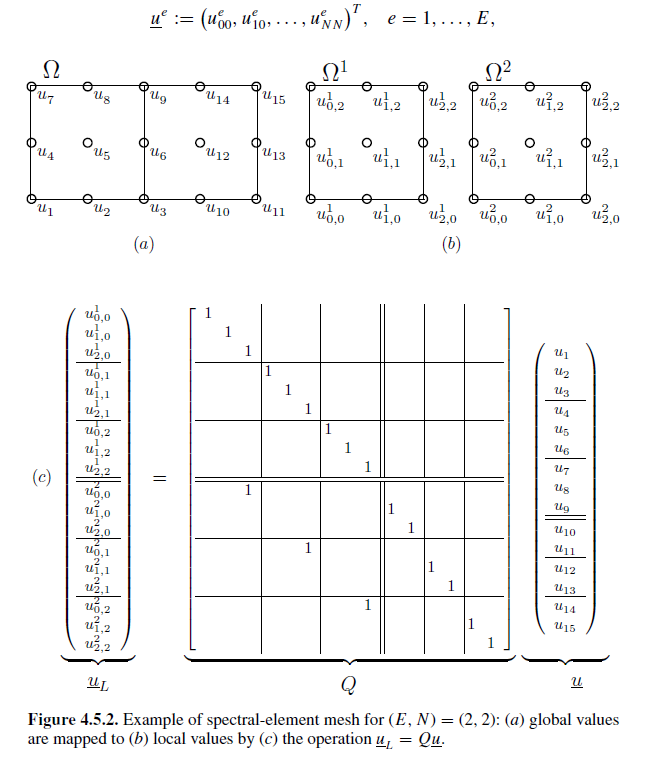
\includegraphics{figs/ac1478334cdfb6c40bd089302ca686c9a0b9eae5.png}

The exact procedure to generate global matrices can be performed for in
3D as in 1D:

\begin{itemize}
\tightlist
\item
  Create unassembled matrices.
\item
  Apply direct stiffness sumation.
\end{itemize}

However this is not done in practice, as the number of operations and
memory requirements are very big. Instead each element is solved
individually and the results are shared by means of gather-scatter
operations.

\hypertarget{implementation-matrix-free-formulation}{%
\section{Implementation: Matrix Free
Formulation}\label{implementation-matrix-free-formulation}}

\emph{Reference: See sections 8.1 - 8.3 in \citet{Deville} }

In the previous sections we learned how tensor products formally
represented on paper. Tensor products are required for evaluation of
spectral operators, but it is not feasible to form large assembled
global matrices, because global matrix operations are memory- and
performance-wise \emph{expensive}. Instead we use:

\begin{itemize}
\tightlist
\item
  \textbf{Local matrix-vector products}, for example the diffusion term:
  \[\mathcal{A^e}=\underline{v^e}^{T}K^e\underline{u^e}\]
  \emph{vectorizable}, and CPU bounded.
\item
  \textbf{Direct stiffness summation}: consecutive gather (\(Q^T\)) and
  scatter (\(Q\)) \[\mathcal{A_L} = Q Q^T \mathcal{A^e}\]
  \emph{communications}, and memory bandwidth bounded.
\end{itemize}

thus, simplifying the operation to a two-step procedure.

\hypertarget{short-detour-vectorization-and-performance}{%
\subsubsection{Short detour: Vectorization and
performance}\label{short-detour-vectorization-and-performance}}

Let us have a quick look at how to avoid common pitfalls to favour
vectorization. Compilers are smart and capable of vectorizing loops,
provided:

\begin{itemize}
\item
  Dependencies are avoided, e.g.: backward substitution of a tridiagonal
  solver

\begin{lstlisting}[language=Fortran]
do i = n-1, 1, -1
   x(i) = (b(i) - u(i) * x(i+1)) / d(i)
enddo
\end{lstlisting}

  would be \emph{much slower} than something like

\begin{lstlisting}[language=Fortran]
do i = 1, n
   x(i) = a(i) + b(i)
enddo
\end{lstlisting}
\item
  Branching avoided: subroutines, functions,
  \passthrough{\lstinline!if!} statements, I/O
\item
  Data locality: strides in memory are aligned with cache lines
\end{itemize}

\hypertarget{example-of-3d-gradient-computation-in-nek5000}{%
\subsection{Example of 3D gradient computation in
Nek5000}\label{example-of-3d-gradient-computation-in-nek5000}}

To demonstrate all these concepts we take a look at how a gradient of
any array is computed in Nek5000. Let us recall that derivatives in each
directions are:

\begin{itemize}
\tightlist
\item
  defined as tensor products \((I \otimes I \otimes D) \underline u^e\),
  etc\ldots{}
\item
  implemented as matrix-matrix multiplications
  \(\Sigma_p D_{ip}u^e_{pjk}\)
\end{itemize}

This ensures data locality and vectorization. To compute the gradient of
an array, the function \passthrough{\lstinline!gradm1!} (see the file in
\passthrough{\lstinline!Nek5000/core/navier5.f!}) is often employed.
This function ultimately calls the matrix-matrix multiplication
\passthrough{\lstinline!mxm!} subroutine:

\begin{lstlisting}[language=Fortran]
       subroutine gradm1(ux,uy,uz,u)
 c
 c     Compute gradient of T -- mesh 1 to mesh 1 (vel. to vel.)
 c     Output: ux, uy, uz  | Input: u
 c
       include 'SIZE'
       include 'DXYZ'
       include 'GEOM'
       include 'INPUT'
       include 'TSTEP'
 c
       parameter(lxyz=lx1*ly1*lz1)
 
       real ux(lxyz,1),uy(lxyz,1),uz(lxyz,1),u(lxyz,1)
 
       ! Scratch arrays
       common /ctmp1/ ur(lxyz),us(lxyz),ut(lxyz)
 
       integer e
 
       nxyz = lx1*ly1*lz1
       ntot = nxyz*nelt
 
       n = lx1-1
       do e=1,nelt
          if (if3d) then
             call local_grad3(ur,us,ut,u,n,e,dxm1,dxtm1)
             do i=1,lxyz
                ux(i,e) = jacmi(i,e)*(ur(i)*rxm1(i,1,1,e)
      $                             + us(i)*sxm1(i,1,1,e)
      $                             + ut(i)*txm1(i,1,1,e) )
                uy(i,e) = jacmi(i,e)*(ur(i)*rym1(i,1,1,e)
      $                             + us(i)*sym1(i,1,1,e)
      $                             + ut(i)*tym1(i,1,1,e) )
                uz(i,e) = jacmi(i,e)*(ur(i)*rzm1(i,1,1,e)
      $                             + us(i)*szm1(i,1,1,e)
      $                             + ut(i)*tzm1(i,1,1,e) )
          else
             ...
       enddo
 c
       return
       end
\end{lstlisting}

For the 3-D case the gradient is \emph{locally} evaluated with a
matrices of shape \passthrough{\lstinline!(lx1, lx1, lx1)!}. Note that
\passthrough{\lstinline!lx1 = m1 = n+1!} is the polynomial order plus 1
to include element boundaries. Within the subroutine
\passthrough{\lstinline!local\_grad3!} the derivative matrices \(D\) and
\(D^T\) are multiplied against a single element of the \(u\) array using
subroutine \passthrough{\lstinline!mxm!}.

\begin{lstlisting}[language=Fortran]
       subroutine local_grad3(ur,us,ut,u,N,e,D,Dt)
 c     Output: ur,us,ut         Input:u,N,e,D,Dt
       real ur(0:n,0:n,0:n),us(0:n,0:n,0:n),ut(0:n,0:n,0:n)
       real u (0:n,0:n,0:n,1)
       real D (0:n,0:n),Dt(0:n,0:n)
       integer e
 c
       m1 = n+1
       m2 = m1*m1
 c
       call mxm(d ,m1,u(0,0,0,e),m1,ur,m2)
       do k=0,n
          call mxm(u(0,0,k,e),m1,dt,m1,us(0,0,k),m1)
       enddo
       call mxm(u(0,0,0,e),m2,dt,m1,ut,m1)
 c
       return
       end
\end{lstlisting}

The matrices \(D\) and \(D^T\) are initialized once and stored in the
include file \passthrough{\lstinline!DXYZ!} within a common block. In
\passthrough{\lstinline!navier1.f!} we find the code responsible for
generating these operators.

\begin{lstlisting}[language=Fortran]
       subroutine get_dgll_ptr (ip,mx,md)
 c
 c     Get pointer to GLL-GLL interpolation dgl() for pair (mx,md)
 c
       include 'SIZE'
 
 c     dgradl holds GLL-based derivative / interpolation operators
 
       parameter(ldg=lxd**3,lwkd=4*lxd*lxd)
       common /dgradl/ d(ldg),dt(ldg),dg(ldg),dgt(ldg),jgl(ldg),jgt(ldg)
      $             , wkd(lwkd)
       
       if (ip.eq.0) then
       ...
          call gen_dgll(d(ip),dt(ip),md,mx,wkd)
       ...
       return
       end
 c-----------------------------------------------------------------------
       subroutine gen_dgll(dgl,dgt,mp,np,w)
 c
 c     Generate derivative from np GL points onto mp GL points
 c
 c        dgl  = derivative matrix, mapping from velocity nodes to pressure
 c        dgt  = transpose of derivative matrix
 c        w    = work array of size (3*np+mp)
 c
 c        np   = number of points on GLL grid
 c        mp   = number of points on GL  grid
 c
 c
 c
       real dgl(mp,np),dgt(np*mp),w(1)
 c
 c
       iz = 1
       id = iz + np
 c
       call zwgll (w(iz),dgt,np)  ! GL points
       call zwgll (w(id),dgt,mp)  ! GL points
 c
       ndgt = 2*np
       ldgt = mp*np
       call lim_chk(ndgt,ldgt,'ldgt ','dgt  ','gen_dgl   ')
 c
       n  = np-1
       do i=1,mp
          call fd_weights_full(w(id+i-1),w(iz),n,1,dgt) ! 1=1st deriv.
          do j=1,np
             dgl(i,j) = dgt(np+j)                       ! Derivative matrix
          enddo
       enddo
 c
       call transpose(dgt,np,dgl,mp)
 c
       return
       end
\end{lstlisting}

The subroutine \passthrough{\lstinline!mxm!} is responsible for
matrix-matrix multiplication and has several optimized implementations
in the file \passthrough{\lstinline!Nek5000/core/mxm\_wrapper.f!}:

\begin{lstlisting}[language=Fortran]
       subroutine mxm(a,n1,b,n2,c,n3)
 c
 c     Compute matrix-matrix product C = A*B
 c     for contiguously packed matrices A,B, and C.
 c
       real a(n1,n2),b(n2,n3),c(n1,n3)
 c
       ...
 
 #ifdef BGQ
       ! Uses IBM Blue Gene specific subroutines
       ...
       goto 111
 #endif
 
 #ifdef XSMM
       ! Uses LIBXSMM: a library for dense and sparse matrix operations
       ...
       goto 111
 #endif
 
 #ifdef BLAS_MXM
       ! Uses the BLAS library bundled with Nek5000 / provided at compile-time
       call dgemm('N','N',n1,n3,n2,1.0,a,n1,b,n2,0.0,c,n1)
       goto 111
 #endif
 
       ! Uses the loop-unrolled matrix multiplication subroutines in mxm_std.f
  101  call mxmf2(a,n1,b,n2,c,n3)
 
  111  continue
       ...
       return
       end
\end{lstlisting}

If \passthrough{\lstinline!n2 = 4!} the \passthrough{\lstinline!mxf4!}
would be called by \passthrough{\lstinline!mxmf2!} (see
\passthrough{\lstinline!Nek5000/core/mxm\_std.f!})

\begin{lstlisting}[language=Fortran]
       subroutine mxf4(a,n1,b,n2,c,n3)
 c
       real a(n1,4),b(4,n3),c(n1,n3)
 c
       do j=1,n3
          do i=1,n1
             c(i,j) = a(i,1)*b(1,j)
      $             + a(i,2)*b(2,j)
      $             + a(i,3)*b(3,j)
      $             + a(i,4)*b(4,j)
          enddo
       enddo
       return
       end
\end{lstlisting}

\hypertarget{back-to-nek5000corenavier5.f-local_grad3}{%
\subsubsection{\texorpdfstring{Back to \texttt{Nek5000/core/navier5.f}:
\texttt{local\_grad3}}{Back to Nek5000/core/navier5.f: local\_grad3}}\label{back-to-nek5000corenavier5.f-local_grad3}}

We compute all three derivatives on a 3-D matrix \(u_{(m,m,m)}\)

\begin{figure}
\centering
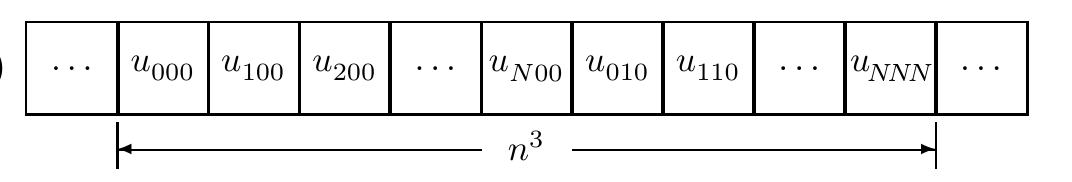
\includegraphics[width=0.5\textwidth,height=\textheight]{figs/8d711f2db9c30e0864b2038788e4e8c30648ad26.png}
\caption{Interpretation of 3D data array as a contiguous vector in
memory}
\end{figure}

\hypertarget{st-mxm}{%
\paragraph{\texorpdfstring{1st \texttt{mxm}}{1st mxm}}\label{st-mxm}}

\(u_r = (I \otimes I \otimes \hat{D}) = \hat{D}_{(m, m)} u_{(m, m^2)}\)

\begin{lstlisting}[language=Fortran]
subroutine local_grad3(ur,us,ut,u,N,e,D,Dt)
Output: ur,us,ut         Input:u,N,e,D,Dt
...
m1 = n+1
m2 = m1*m1

call mxm(d ,m1,u(0,0,0,e),m1,ur,m2)
...
\end{lstlisting}

\begin{figure}
\centering
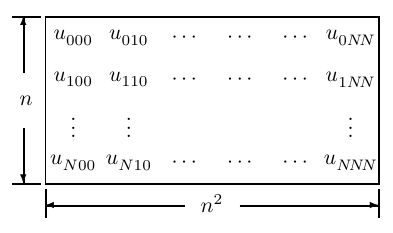
\includegraphics[width=0.5\textwidth,height=\textheight]{figs/b7cef4a74c1cb5eb009b3d833f658ba806965cab.png}
\caption{Interpretation of 3D data array as a \(n \times n^2\) matrix}
\end{figure}

\hypertarget{nd-mxm}{%
\paragraph{\texorpdfstring{2nd \texttt{mxm}}{2nd mxm}}\label{nd-mxm}}

\(u_{s} = I \otimes \hat{D} \otimes I = u_{(m, m)} \hat{D}^T_{(m, m)}\)

\begin{lstlisting}[language=Fortran]
subroutine local_grad3(ur,us,ut,u,N,e,D,Dt)
Output: ur,us,ut         Input:u,N,e,D,Dt
...
m1 = n+1
m2 = m1*m1
...
do k=0,n
   call mxm(u(0,0,k,e),m1,dt,m1,us(0,0,k),m1)
enddo
...
\end{lstlisting}

\begin{figure}
\centering
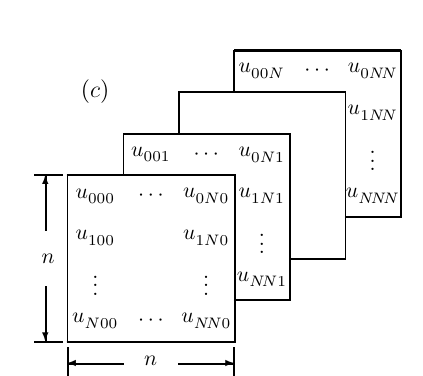
\includegraphics[width=0.5\textwidth,height=\textheight]{figs/c8583cc0161a26f00fca48847ad5cebd79ea0e65.png}
\caption{Interpretation of 3D data array as a sequence of \(n\)
\(n \times n\) matrices}
\end{figure}

\hypertarget{rd-mxm}{%
\paragraph{\texorpdfstring{3rd \texttt{mxm}}{3rd mxm}}\label{rd-mxm}}

\(u_{t} = \hat{D} \otimes I \otimes I = u_{(m^2, m)} \hat{D}^T_{(m, m)}\)

\begin{lstlisting}[language=Fortran]
subroutine local_grad3(ur,us,ut,u,N,e,D,Dt)
Output: ur,us,ut         Input:u,N,e,D,Dt
...
m1 = n+1
m2 = m1*m1
...
call mxm(u(0,0,0,e),m2,dt,m1,ut,m1)

return
end
\end{lstlisting}

\begin{figure}
\centering
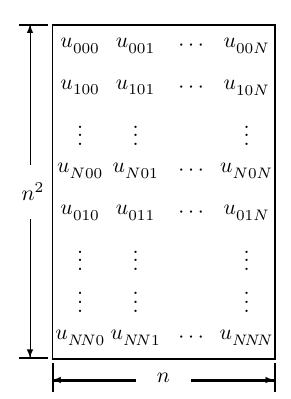
\includegraphics[width=0.5\textwidth,height=\textheight]{figs/42abdb01633a6d4d696312b5360e89d4b3854b97.png}
\caption{Interpretation of 3D data array as a \(n^2 \times n\) matrix}
\end{figure}

  \bibliography{references.bib}

\end{document}
